\documentclass[aspectratio=169]{beamer}
\usetheme{Madrid}
\usecolortheme{default}

\usepackage[utf8]{inputenc}
\usepackage[T1]{fontenc}
\usepackage{graphicx}
\usepackage{tikz}
\usepackage{listings}
\usepackage{hyperref}
\usepackage{fontawesome5}
\usepackage{amssymb}

\usetikzlibrary{shapes.geometric, arrows, positioning, shadows, calc}

\definecolor{kivablue}{RGB}{41, 128, 185}
\definecolor{kivagreen}{RGB}{39, 174, 96}
\definecolor{kivaorange}{RGB}{230, 126, 34}
\definecolor{kivared}{RGB}{231, 76, 60}
\definecolor{kivagray}{RGB}{127, 140, 141}

\setbeamercolor{structure}{fg=kivablue}
\setbeamercolor{palette primary}{bg=kivablue,fg=white}
\setbeamercolor{palette secondary}{bg=kivagreen,fg=white}
\setbeamercolor{palette tertiary}{bg=kivaorange,fg=white}
\setbeamercolor{palette quaternary}{bg=kivared,fg=white}

\lstset{
    basicstyle=\ttfamily\footnotesize,
    breaklines=true,
    frame=single,
    backgroundcolor=\color{gray!10},
    literate={"}{\textquotedbl}1
}

\title[KIVA Pre-Session]{Building AI Tutors with KIVA}
\subtitle{MA AI Hub x SundAI — Reimagining Education with AI}
\author{Hack Day Pre-Session}
\date{May 6, 2026}
\institute{MIT AI Hub}

\begin{document}

\begin{frame}
\titlepage
\end{frame}

\begin{frame}{Outline}
\tableofcontents
\end{frame}

\section{Event Overview}

\begin{frame}{MA AI Hub x SundAI Hack Day}
\begin{block}{Mission}
Explore how AI can reshape learning through hands-on prototyping
\end{block}

\vspace{0.5cm}

\begin{columns}[T]
\column{0.5\textwidth}
\textbf{Schedule}
\begin{itemize}
    \item \textcolor{kivablue}{\textbf{Pre-session:}} May 6, 6:00-7:30 PM
    \item \textcolor{kivagreen}{\textbf{Hack Day:}} May 9, 9:00 AM-5:00 PM
\end{itemize}

\column{0.5\textwidth}
\textbf{Who Should Join}
\begin{itemize}
    \item Educators
    \item Researchers
    \item Developers \& AI builders
    \item Students
\end{itemize}
\end{columns}
\end{frame}

\begin{frame}{Focus Areas}
\begin{enumerate}
    \item \textbf{\textcolor{kivablue}{AI Tutors — Build on KIVA}}
    \begin{itemize}
        \item Evaluate tutor behavior in real scenarios
        \item Prototype improvements: feedback flows, personalization, safety
        \item Analyze educator interaction and intervention points
    \end{itemize}
    
    \vspace{0.3cm}
    
    \item \textbf{\textcolor{kivagreen}{Learning Path Engines}}
    \begin{itemize}
        \item Generate personalized learning pathways
        \item Sequence real content (papers, courses)
        \item Adapt to learner background
    \end{itemize}
    
    \vspace{0.3cm}
    
    \item \textbf{\textcolor{kivaorange}{Future of Education Systems}}
    \begin{itemize}
        \item Build educator tools
        \item Create new learning experiences
        \item Push education forward
    \end{itemize}
\end{enumerate}
\end{frame}

\section{What is KIVA?}

\begin{frame}{KIVA: Knowledge Integration \& Vocabulary Acquisition}
\begin{block}{Definition}
KIVA is an \textbf{open-source AI tutoring platform} built on Riverst that enables interactive, speech-driven learning experiences with AI avatars.
\end{block}

\vspace{0.5cm}

\begin{columns}[T]
\column{0.5\textwidth}
\textbf{Key Features}
\begin{itemize}
    \item \faRobot\ Real-time avatar interaction
    \item \faMicrophone\ Speech-based conversations
    \item \faChartLine\ Automated analysis
    \item \faCogs\ Customizable flows
    \item \faDatabase\ Session recording
\end{itemize}

\column{0.5\textwidth}
\textbf{Use Cases}
\begin{itemize}
    \item Vocabulary tutoring
    \item Language learning (ESL/ISL)
    \item Audiobook comprehension
    \item Custom educational activities
\end{itemize}
\end{columns}
\end{frame}

\begin{frame}{KIVA Demo Videos}
\begin{itemize}
    \item \textbf{Riverst Platform Demo}
    \begin{itemize}
        \item Overview of capabilities
        \item \url{https://drive.google.com/file/d/1r2LoBGbjBx1mdDIv-fPzGeZVEYf1kLw8/view}
    \end{itemize}
    
    \vspace{0.3cm}
    
    \item \textbf{KIVA Vocabulary Activity}
    \begin{itemize}
        \item Vocabulary teaching workflow demonstration
        \item \url{https://drive.google.com/file/d/1jTHvTXG4WWIYqgqjC4lp1LWMEnyZJQzr/view}
    \end{itemize}
    
    \vspace{0.3cm}
    
    \item \textbf{Activity Summary \& Configuration}
    \begin{itemize}
        \item Configuration pages and automated analysis
        \item \url{https://drive.google.com/file/d/1AvYnSq87neOYj_YSduYatN5D4rdO-7QG/view}
    \end{itemize}
\end{itemize}

\vspace{0.3cm}
\begin{center}
\textcolor{kivablue}{\faInfoCircle\ Watch these before the hack day!}
\end{center}
\end{frame}

\section{System Architecture}

\begin{frame}{How KIVA Works: High-Level Architecture}
\begin{center}
\begin{tikzpicture}[
    node distance=1.5cm,
    box/.style={rectangle, rounded corners, draw=kivablue, fill=kivablue!20, thick, minimum width=2.5cm, minimum height=1cm, align=center, drop shadow},
    arrow/.style={->, >=stealth, thick, color=kivablue}
]

\node[box] (user) {\faUser\ \textbf{User}\\ (Browser)};
\node[box, right=of user] (client) {\faReact\ \textbf{React Client}\\ WebRTC};
\node[box, right=of client] (server) {\faPython\ \textbf{FastAPI Server}\\ Bot Runner};
\node[box, below=of server] (ai) {\faBrain\ \textbf{AI Services}\\ STT/LLM/TTS};
\node[box, left=of ai] (flow) {\faProjectDiagram\ \textbf{Flow Engine}\\ Pipecat};
\node[box, left=of flow] (avatar) {\faRobot\ \textbf{3D Avatar}\\ Three.js};

\draw[arrow] (user) -- (client);
\draw[arrow] (client) -- (server);
\draw[arrow] (server) -- (ai);
\draw[arrow] (ai) -- (flow);
\draw[arrow] (flow) -- (avatar);
\draw[arrow] (avatar) -- (user);

\end{tikzpicture}
\end{center}

\vspace{0.3cm}
\textbf{Real-time Pipeline:} Speech $\rightarrow$ STT $\rightarrow$ LLM $\rightarrow$ TTS $\rightarrow$ Avatar Animation
\end{frame}

\begin{frame}{Activity Lifecycle}
\begin{center}
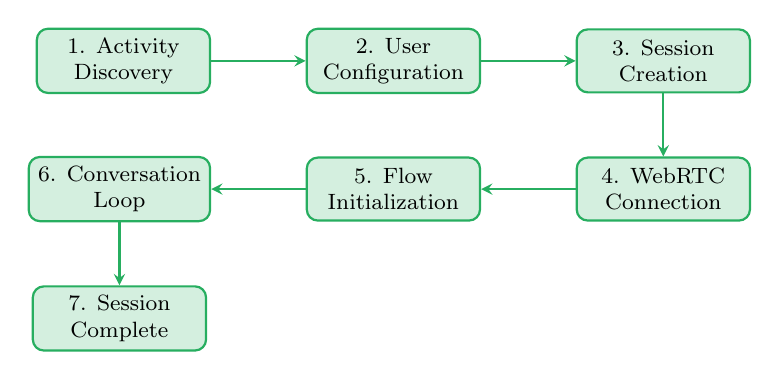
\begin{tikzpicture}[
    node distance=0.8cm and 1.2cm,
    stepnode/.style={rectangle, rounded corners, draw=kivagreen, fill=kivagreen!20, thick, minimum width=2.2cm, minimum height=0.8cm, align=center, font=\footnotesize},
    arrow/.style={->, >=stealth, thick, color=kivagreen}
]

\node[stepnode] (discover) {1. Activity\\Discovery};
\node[stepnode, right=of discover] (config) {2. User\\Configuration};
\node[stepnode, right=of config] (session) {3. Session\\Creation};
\node[stepnode, below=of session] (webrtc) {4. WebRTC\\Connection};
\node[stepnode, left=of webrtc] (flow) {5. Flow\\Initialization};
\node[stepnode, left=of flow] (loop) {6. Conversation\\Loop};
\node[stepnode, below=of loop] (complete) {7. Session\\Complete};

\draw[arrow] (discover) -- (config);
\draw[arrow] (config) -- (session);
\draw[arrow] (session) -- (webrtc);
\draw[arrow] (webrtc) -- (flow);
\draw[arrow] (flow) -- (loop);
\draw[arrow] (loop) -- (complete);

\end{tikzpicture}
\end{center}

\vspace{0.3cm}
\begin{itemize}
    \item Frontend loads activities from \texttt{/api/activities}
    \item User configures via session schema
    \item Backend establishes WebRTC and initializes AI pipeline
    \item Flow system manages conversation state and transitions
\end{itemize}
\end{frame}

\begin{frame}{Core Components}
\begin{columns}[T]
\column{0.5\textwidth}
\textbf{Frontend (React)}
\begin{itemize}
    \item \texttt{Homepage.tsx} — Activity browser
    \item \texttt{AvatarInteractionSettings.tsx} — Config UI
    \item \texttt{AvatarRenderer.tsx} — 3D avatar (Three.js)
    \item WebRTC connection management
\end{itemize}

\vspace{0.5cm}

\textbf{Backend (FastAPI)}
\begin{itemize}
    \item \texttt{main.py} — API endpoints
    \item \texttt{bot\_runner.py} — Orchestration
    \item \texttt{flow\_factory.py} — Flow builder
    \item \texttt{handlers.py} — State management
\end{itemize}

\column{0.5\textwidth}
\textbf{AI Services}
\begin{itemize}
    \item \textbf{STT:} OpenAI Whisper / Local Whisper
    \item \textbf{LLM:} OpenAI GPT / Ollama (local)
    \item \textbf{TTS:} OpenAI TTS
\end{itemize}

\vspace{0.5cm}

\textbf{Flow System (Pipecat)}
\begin{itemize}
    \item Stage progression tracking
    \item Function calling system
    \item Transition logic
    \item Context management
\end{itemize}

\vspace{0.5cm}

\textbf{Analysis (Senselab)}
\begin{itemize}
    \item Speech feature extraction
    \item Behavioral analysis
    \item Automated transcription
\end{itemize}
\end{columns}
\end{frame}

\section{Installation Guide}

\begin{frame}[fragile]{System Requirements}
\begin{block}{Supported Platforms}
\begin{itemize}
    \item \textcolor{kivagreen}{\faCheck} Apple Silicon (M-chip) macOS
    \item \textcolor{kivagreen}{\faCheck} Ubuntu Linux
    \item \textcolor{kivared}{\faTimes} Windows (not supported)
\end{itemize}
\end{block}

\vspace{0.3cm}

\begin{columns}[T]
\column{0.5\textwidth}
\textbf{Software Requirements}
\begin{itemize}
    \item Python 3.11+
    \item Node.js 16+
    \item FFmpeg 7.*
    \item Modern browser (Chrome 134+)
\end{itemize}

\column{0.5\textwidth}
\textbf{API Keys (Optional)}
\begin{itemize}
    \item OpenAI API key
    \item Hugging Face token
    \item Google OAuth (optional)
\end{itemize}
\end{columns}

\vspace{0.3cm}
\begin{alertblock}{Note}
Not all API keys are required. Local models (Ollama, Whisper) can run without external APIs.
\end{alertblock}
\end{frame}

\begin{frame}[fragile]{Installation: Step 1 — Clone Repository}
\begin{verbatim}
# Clone the repository
git clone https://github.com/sensein/riverst.git
cd riverst
\end{verbatim}

\vspace{0.5cm}

\begin{block}{Repository Structure}
\small
\texttt{riverst/} contains \texttt{src/server/} (FastAPI backend), \texttt{src/client/react/} (React frontend), \texttt{KIVA/} (documentation), and \texttt{docker-compose.yaml}
\end{block}
\end{frame}

\begin{frame}{Installation: Step 2 — Environment Setup}
\textbf{Server Configuration}
\begin{itemize}
    \item \texttt{cd src/server}
    \item \texttt{cp env.example .env}
    \item Edit .env and add your API keys
\end{itemize}

\vspace{0.3cm}

\textbf{Client Configuration}
\begin{itemize}
    \item \texttt{cd src/client/react}
    \item \texttt{cp env.example .env}
\end{itemize}

\vspace{0.3cm}

\begin{block}{Minimal .env for Server}
OPENAI\_API\_KEY, HF\_TOKEN, ANALYZE\_AUDIO=true
\end{block}
\end{frame}

\begin{frame}{Installation: Step 3 — Install Dependencies}
\textbf{Option A: Using Conda (Recommended)}
\begin{itemize}
    \item \texttt{conda create -n riverst python=3.11}
    \item \texttt{conda activate riverst}
    \item \texttt{conda install -c conda-forge ffmpeg}
    \item \texttt{pip install -r requirements.txt}
\end{itemize}

\vspace{0.3cm}

\textbf{Option B: Using Docker}
\begin{itemize}
    \item \texttt{docker compose up --build}
\end{itemize}

\vspace{0.3cm}

\textbf{Client setup}
\begin{itemize}
    \item \texttt{cd src/client/react \&\& npm install}
\end{itemize}
\end{frame}

\begin{frame}{Installation: Step 4 — Run KIVA}
\textbf{Start Server (Terminal 1)}
\begin{itemize}
    \item \texttt{cd src/server}
    \item \texttt{conda activate riverst}
    \item \texttt{python main.py}
    \item Server runs on \texttt{http://localhost:7860}
\end{itemize}

\vspace{0.3cm}

\textbf{Start Client (Terminal 2)}
\begin{itemize}
    \item \texttt{cd src/client/react}
    \item \texttt{npm run dev}
    \item Client runs on \texttt{http://localhost:5173}
\end{itemize}

\vspace{0.3cm}

\begin{alertblock}{Important}
\faExclamationTriangle\ The server \textbf{must} be running before starting the client!
\end{alertblock}

\vspace{0.2cm}
\begin{block}{Quick Start Scripts}
Use \texttt{./start\_server.sh} and \texttt{./start\_client.sh} from repo root
\end{block}
\end{frame}

\begin{frame}{Verification}
\begin{enumerate}
    \item Open browser to \texttt{http://localhost:5173}
    \item You should see the Riverst homepage
    \item Look for \textbf{"Knowledge Integration and Vocabulary Acquisition through AI (KIVA)"} section
    \item Try the \textbf{"Child vocabulary training"} activity
\end{enumerate}

\vspace{0.5cm}

\begin{block}{Troubleshooting}
\begin{itemize}
    \item \textbf{Port conflicts:} Check if 7860 or 5173 are in use
    \item \textbf{API errors:} Verify \texttt{.env} has valid OpenAI key
    \item \textbf{FFmpeg missing:} Install via conda or system package manager
    \item \textbf{Browser issues:} Use Chrome 134+ for WebRTC support
\end{itemize}
\end{block}
\end{frame}

\section{Activity Structure}

\begin{frame}{Activity Types}
\begin{columns}[T]
\column{0.5\textwidth}
\textbf{Simple Activities}
\begin{itemize}
    \item Only \texttt{session\_config.json}
    \item Open-ended conversations
    \item No structured flow
    \item Example: \texttt{basic-avatar-demo}
\end{itemize}

\column{0.5\textwidth}
\textbf{Advanced Flow Activities}
\begin{itemize}
    \item \texttt{session\_config.json} + \texttt{flow\_config.json}
    \item Structured conversation stages
    \item Dynamic content adaptation
    \item Example: \texttt{vocab-tutoring}
\end{itemize}
\end{columns}

\vspace{0.5cm}

\begin{block}{For Hack Day}
You'll primarily work with \textbf{advanced flow activities} to build sophisticated tutoring behaviors.
\end{block}
\end{frame}

\begin{frame}{Session Configuration}
\texttt{session\_config.json} defines activity parameters and UI options:

\begin{block}{Key Configuration Fields}
\begin{itemize}
    \item AI service selection (STT/LLM/TTS)
    \item Avatar behavior prompts
    \item UI options (video, transcripts)
    \item Embodiment type (avatar vs waveform)
\end{itemize}
\end{block}

\vspace{0.3cm}
\textbf{Key Fields:}
\begin{itemize}
    \item AI service selection (STT/LLM/TTS)
    \item Avatar behavior prompts
    \item UI options (video, transcripts)
\end{itemize}
\end{frame}

\begin{frame}{Flow Configuration}
\texttt{flow\_config.json} defines conversation structure:

\begin{block}{Flow Elements}
\begin{itemize}
    \item \textbf{Nodes:} Conversation stages (greeting, teaching, review, end)
    \item \textbf{Transitions:} Movement between stages based on conditions
    \item \textbf{Actions:} Custom Python handlers (pre/post)
    \item \textbf{Role messages:} System prompts for each stage
\end{itemize}
\end{block}

\vspace{0.3cm}
\textbf{Flow Elements:}
\begin{itemize}
    \item \textbf{Nodes:} Conversation stages
    \item \textbf{Transitions:} Movement between stages
    \item \textbf{Actions:} Custom Python handlers (pre/post)
\end{itemize}
\end{frame}

\section{Learning Verification Without Data Storage}

\begin{frame}{How Does KIVA Know Learning Happens?}
\begin{alertblock}{Privacy-First Approach}
KIVA can verify learning \textbf{without storing any personal data}
\end{alertblock}

\vspace{0.3cm}

\begin{columns}[T]
\column{0.5\textwidth}
\textbf{What KIVA Does NOT Store:}
\begin{itemize}
    \item No user profiles
    \item No learning history
    \item No persistent data
    \item No cross-session tracking
\end{itemize}

\column{0.5\textwidth}
\textbf{What KIVA CAN Verify:}
\begin{itemize}
    \item In-session progress
    \item Real-time comprehension
    \item Immediate application
    \item Session-end mastery
\end{itemize}
\end{columns}
\end{frame}

\begin{frame}{Strategy 1: Contextual Memory (LLM)}
\textbf{The LLM remembers the entire conversation in its context window:}

\vspace{0.3cm}

\begin{center}
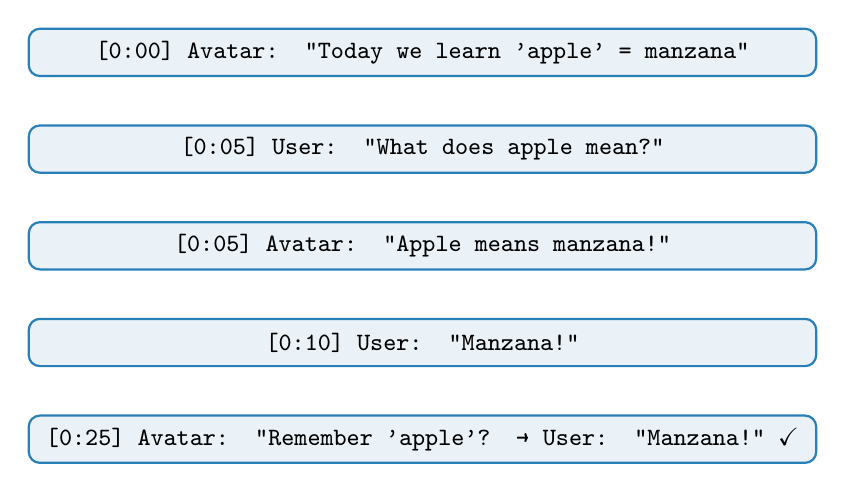
\begin{tikzpicture}[
    node distance=0.6cm,
    msgbox/.style={rectangle, rounded corners, draw=kivablue, fill=kivablue!10, thick, minimum width=10cm, minimum height=0.6cm, align=left, font=\small}
]
\node[msgbox] (m1) {\texttt{[0:00] Avatar: "Today we learn 'apple' = manzana"}};
\node[msgbox, below=of m1] (m2) {\texttt{[0:05] User: "What does apple mean?"}};
\node[msgbox, below=of m2] (m3) {\texttt{[0:05] Avatar: "Apple means manzana!"}};
\node[msgbox, below=of m3] (m4) {\texttt{[0:10] User: "Manzana!"}};
\node[msgbox, below=of m4] (m5) {\texttt{[0:25] Avatar: "Remember 'apple'? → User: "Manzana!" \checkmark}};
\end{tikzpicture}
\end{center}

\vspace{0.3cm}

\begin{block}{Verification}
The LLM can quiz on earlier content \textbf{anytime during the session}
\end{block}
\end{frame}

\begin{frame}{Strategy 2: Session State Tracking}
\textbf{Temporary state maintained only during active session:}

\vspace{0.3cm}

\begin{columns}[T]
\column{0.5\textwidth}
\begin{block}{Session State (Ephemeral)}
\footnotesize
\texttt{\{}\\
\texttt{~~"words\_introduced": 5,}\\
\texttt{~~"words\_correct": 4,}\\
\texttt{~~"words\_failed": 1,}\\
\texttt{~~"current\_difficulty": 2}\\
\texttt{\}}
\end{block}

\column{0.5\textwidth}
\textbf{Enables Real-Time:}
\begin{itemize}
    \item Progress tracking
    \item Difficulty adaptation
    \item Spaced repetition
    \item Mastery detection
\end{itemize}
\end{columns}

\vspace{0.3cm}

\begin{alertblock}{Key Point}
State is \textbf{deleted} when session ends — no persistence
\end{alertblock}
\end{frame}

\begin{frame}{Strategy 3: Progressive Verification}
\textbf{Bloom's Taxonomy applied within a single session:}

\vspace{0.3cm}

\begin{center}
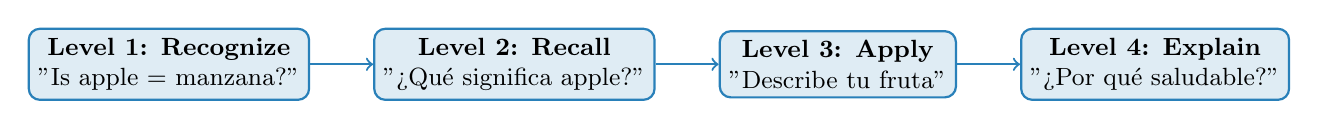
\begin{tikzpicture}[
    node distance=0.8cm,
    levelbox/.style={rectangle, rounded corners, draw=kivablue, fill=kivablue!15, thick, minimum width=3cm, minimum height=0.8cm, align=center, font=\small}
]
\node[levelbox] (l1) {\textbf{Level 1: Recognize}\\"Is apple = manzana?"};
\node[levelbox, right=of l1] (l2) {\textbf{Level 2: Recall}\\"¿Qué significa apple?"};
\node[levelbox, right=of l2] (l3) {\textbf{Level 3: Apply}\\"Describe tu fruta"};
\node[levelbox, right=of l3] (l4) {\textbf{Level 4: Explain}\\"¿Por qué saludable?"};

\draw[->, thick, kivablue] (l1) -- (l2);
\draw[->, thick, kivablue] (l2) -- (l3);
\draw[->, thick, kivablue] (l3) -- (l4);
\end{tikzpicture}
\end{center}

\vspace{0.3cm}

\begin{block}{How It Works}
Each level builds on previous — if student fails Level 3, avatar knows they passed Level 2 but need more practice
\end{block}
\end{frame}

\begin{frame}{Strategy 4: Spaced Repetition (In-Session)}
\textbf{Testing at increasing intervals within same session:}

\vspace{0.3cm}

\begin{center}
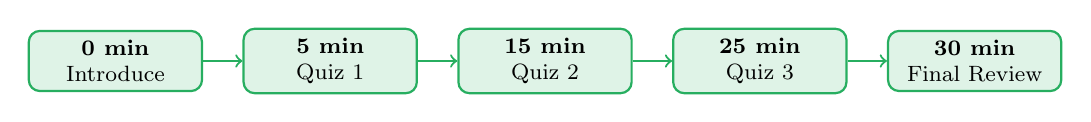
\begin{tikzpicture}[
    node distance=0.5cm,
    timebox/.style={rectangle, rounded corners, draw=kivagreen, fill=kivagreen!15, thick, minimum width=2.2cm, minimum height=0.7cm, align=center, font=\footnotesize}
]
\node[timebox] (t0) {\textbf{0 min}\\Introduce};
\node[timebox, right=of t0] (t1) {\textbf{5 min}\\Quiz 1};
\node[timebox, right=of t1] (t2) {\textbf{15 min}\\Quiz 2};
\node[timebox, right=of t2] (t3) {\textbf{25 min}\\Quiz 3};
\node[timebox, right=of t3] (t4) {\textbf{30 min}\\Final Review};

\draw[->, thick, kivagreen] (t0) -- (t1);
\draw[->, thick, kivagreen] (t1) -- (t2);
\draw[->, thick, kivagreen] (t2) -- (t3);
\draw[->, thick, kivagreen] (t3) -- (t4);
\end{tikzpicture}
\end{center}

\vspace{0.3cm}

\begin{columns}[T]
\column{0.5\textwidth}
\textbf{If Correct:}
\begin{itemize}
    \item Increase interval
    \item Move to next concept
\end{itemize}

\column{0.5\textwidth}
\textbf{If Incorrect:}
\begin{itemize}
    \item Provide remediation
    \item Re-test sooner
\end{itemize}
\end{columns}
\end{frame}

\begin{frame}{Strategy 5: Real-Time Pattern Detection}
\textbf{Analyzing user behavior during conversation:}

\vspace{0.3cm}

\begin{columns}[T]
\column{0.5\textwidth}
\begin{block}{Behavioral Signals}
\begin{itemize}
    \item \textbf{Hesitation} — Long pauses before answering
    \item \textbf{Self-correction} — "Wait, I mean..."
    \item \textbf{Confidence} — Voice tone, speed
    \item \textbf{Accuracy} — Correct vs incorrect responses
\end{itemize}
\end{block}

\column{0.5\textwidth}
\begin{block}{Adaptive Response}
\begin{itemize}
    \item Slow down if hesitation
    \item Provide hints if struggling
    \item Challenge if confident
    \item Celebrate if accurate
\end{itemize}
\end{block}
\end{columns}

\vspace{0.3cm}

\begin{alertblock}{Example}
If user pauses 5+ seconds → Avatar: "Take your time, here's a hint..."
\end{alertblock}
\end{frame}

\begin{frame}{Session Summary (No Storage Required)}
\textbf{At session end, KIVA generates a summary:}

\vspace{0.3cm}

\begin{block}{Example Summary}
\small
"Today's session covered:\\
\quad \checkmark{} 5 vocabulary words introduced\\
\quad \checkmark{} 4 mastered on first try\\
\quad \checkmark{} 1 needed 3 attempts (orange)\\[0.2cm]
\textbf{Recommendation:} Review 'orange' in next session"
\end{block}

\vspace{0.3cm}

\begin{columns}[T]
\column{0.5\textwidth}
\textbf{User Options:}
\begin{itemize}
    \item Download summary as PDF
    \item Email to themselves
    \item Copy to notes
    \item Share with teacher
\end{itemize}

\column{0.5\textwidth}
\textbf{Privacy Benefits:}
\begin{itemize}
    \item User controls their data
    \item Nothing stored on server
    \item GDPR compliant
    \item No consent needed
\end{itemize}
\end{columns}
\end{frame}

\begin{frame}{Trade-offs: No Persistent Storage}
\begin{columns}[T]
\column{0.5\textwidth}
\textbf{\textcolor{kivagreen}{\faCheck{} Advantages}}
\begin{itemize}
    \item Complete privacy
    \item GDPR compliant by default
    \item No data breaches possible
    \item Simpler infrastructure
    \item Works offline
    \item No consent management
\end{itemize}

\column{0.5\textwidth}
\textbf{\textcolor{kivared}{\faTimes{} Limitations}}
\begin{itemize}
    \item No long-term progress tracking
    \item Each session starts fresh
    \item No personalized curriculum
    \item No cross-session adaptation
    \item User must track own progress
\end{itemize}
\end{columns}

\vspace{0.3cm}

\begin{block}{Hybrid Approach (Optional)}
Allow users to \textbf{opt-in} to long-term memory for personalized learning
\end{block}
\end{frame}

\section{Hack Day Opportunities}

\begin{frame}{What You Can Build}
\begin{block}{Evaluation \& Analysis}
\begin{itemize}
    \item Analyze tutor behavior in real scenarios
    \item Study conversation logs and patterns
    \item Identify where the AI breaks down
    \item Determine when human intervention is needed
\end{itemize}
\end{block}

\vspace{0.3cm}

\begin{block}{Prototype Improvements}
\begin{itemize}
    \item \textbf{Feedback flows:} Better assessment and correction
    \item \textbf{Personalization:} Adapt to learner level and style
    \item \textbf{Intervention checkpoints:} When to alert educators
    \item \textbf{Analytics dashboards:} Track progress and engagement
    \item \textbf{Safety layers:} Content filtering and guardrails
    \item \textbf{Educator controls:} Tools for teachers to guide sessions
\end{itemize}
\end{block}
\end{frame}

\begin{frame}{Example Projects}
\begin{enumerate}
    \item \textbf{Adaptive Difficulty System}
    \begin{itemize}
        \item Monitor student performance in real-time
        \item Adjust vocabulary complexity dynamically
        \item Implement spaced repetition
    \end{itemize}
    
    \vspace{0.3cm}
    
    \item \textbf{Educator Dashboard}
    \begin{itemize}
        \item Live session monitoring
        \item Intervention triggers (student struggling)
        \item Post-session analytics and insights
    \end{itemize}
    
    \vspace{0.3cm}
    
    \item \textbf{Multi-Modal Assessment}
    \begin{itemize}
        \item Analyze speech patterns (pronunciation, fluency)
        \item Track engagement via video (attention, emotion)
        \item Combine metrics for holistic evaluation
    \end{itemize}
    
    \vspace{0.3cm}
    
    \item \textbf{Safety \& Content Filtering}
    \begin{itemize}
        \item Detect inappropriate content
        \item Age-appropriate language adaptation
        \item Bias detection and mitigation
    \end{itemize}
\end{enumerate}
\end{frame}

\begin{frame}{Technical Extension Points}
\begin{columns}[T]
\column{0.5\textwidth}
\textbf{Backend Extensions}
\begin{itemize}
    \item Custom handlers in \texttt{handlers.py}
    \item New flow configurations
    \item Additional AI service integrations
    \item Database for learner profiles
    \item Real-time analytics pipeline
\end{itemize}

\vspace{0.3cm}

\textbf{Frontend Extensions}
\begin{itemize}
    \item New activity configuration UIs
    \item Live session monitoring
    \item Educator dashboards
    \item Student progress views
\end{itemize}

\column{0.5\textwidth}
\textbf{Flow System Extensions}
\begin{itemize}
    \item Branching logic based on performance
    \item Dynamic content loading
    \item Multi-stage assessments
    \item Personalization algorithms
\end{itemize}

\vspace{0.3cm}

\textbf{Analysis Extensions}
\begin{itemize}
    \item Custom Senselab pipelines
    \item Speech quality metrics
    \item Engagement detection
    \item Learning outcome prediction
\end{itemize}
\end{columns}

\vspace{0.5cm}
\begin{alertblock}{Tip}
Start with flow modifications — they're the fastest way to prototype new behaviors!
\end{alertblock}
\end{frame}

\section{Resources \& Next Steps}

\begin{frame}{Documentation \& Resources}
\begin{itemize}
    \item \textbf{GitHub Repository:} \url{https://github.com/sensein/riverst}
    \item \textbf{Activity Creation Guide:} \texttt{src/server/activities/ACTIVITY\_CREATION\_GUIDE.md}
    \item \textbf{Project Board:} \url{https://github.com/orgs/sensein/projects/55}
    \item \textbf{Pipecat Framework:} \url{https://github.com/pipecat-ai/pipecat}
    \item \textbf{Senselab:} \url{https://github.com/sensein/senselab}
\end{itemize}

\vspace{0.5cm}

\begin{block}{Before Hack Day}
\begin{enumerate}
    \item Install KIVA and verify it runs
    \item Watch the demo videos
    \item Explore the \texttt{vocab-tutoring} activity
    \item Read the Activity Creation Guide
    \item Think about what you want to build!
\end{enumerate}
\end{block}
\end{frame}

\begin{frame}{Getting Help}
\begin{columns}[T]
\column{0.5\textwidth}
\textbf{During Pre-Session (May 6)}
\begin{itemize}
    \item Installation troubleshooting
    \item Architecture questions
    \item Project ideation
    \item Team formation
\end{itemize}

\column{0.5\textwidth}
\textbf{During Hack Day (May 9)}
\begin{itemize}
    \item Technical support
    \item Code reviews
    \item Integration help
    \item Demo preparation
\end{itemize}
\end{columns}

\vspace{0.5cm}

\begin{block}{Communication Channels}
\begin{itemize}
    \item Event Slack/Discord (TBD)
    \item GitHub Issues for bugs
    \item In-person mentors on hack day
\end{itemize}
\end{block}
\end{frame}

\begin{frame}{Quick Reference: Key Commands}
\begin{block}{Installation}
\small
\texttt{git clone https://github.com/sensein/riverst.git}\\
\texttt{conda create -n riverst python=3.11}\\
\texttt{conda activate riverst}\\
\texttt{pip install -r requirements.txt}
\end{block}

\begin{block}{Running}
\small
Terminal 1: \texttt{python main.py} (in src/server)\\
Terminal 2: \texttt{npm run dev} (in src/client/react)
\end{block}

\begin{block}{Access}
\begin{itemize}
    \item Frontend: \texttt{http://localhost:5173}
    \item Backend API: \texttt{http://localhost:7860}
\end{itemize}
\end{block}
\end{frame}

\begin{frame}
\begin{center}
\Huge Questions?

\vspace{1cm}

\Large Let's build the future of education together!

\vspace{1cm}

\normalsize
\faGithub\ \url{https://github.com/sensein/riverst}

\vspace{0.3cm}

See you on May 9!
\end{center}
\end{frame}

\end{document}
